\documentclass[tikz]{standalone}
\begin{document}
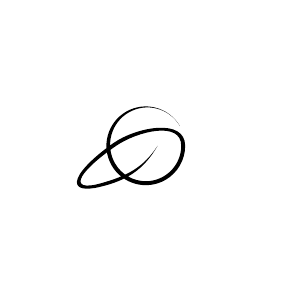
\begin{tikzpicture}
\useasboundingbox (-1.5,-1.5) rectangle (1.5,1.5);

%% Help lines
% \begin{scope}[help lines, opacity=0.1]
%     \draw[step=0.1] (-1.45,-1.45) grid (1.45,1.45);
%     \draw[thin] (-1.5,0) -- (1.5,0) (0,-1.5) -- (0,1.5);
%     \draw circle (1.5);
% \end{scope}

%% Planet
\begin{scope}[rotate=30]
    %% Basic construction
    % \begin{scope}[help lines]
    %     \draw (0,0) circle [radius=0.5];
    %     \draw (0:0.025) circle [radius=0.475];
    %     \draw (0,0) circle [radius=0.45];
    %     \draw (0,0) ellipse [x radius=1, y radius=0.25];
    %     \draw (0,0) ellipse [x radius=0.95, y radius=0.20];
        
    %     \draw
    %         (0:0.5)
    %         arc (0:330:0.5)
    %         to [out=60, in=5.2] (110:1 and 0.25)
    %         arc (110:220:1 and 0.25)
    %         to [out=-16.6, in=210] (-30:.15);
    % \end{scope}

    \fill
        (0:0.5)
        arc (0:330:0.5)
        to [out=60, in=5.2] (110:1 and 0.25)
        arc (110:220:1 and 0.25)
        to [out=-16.6, in=210] (-30:.15)
        coordinate (tip)
        to [out=207, in=-14.1] (220:0.95 and 0.20)
        arc (220:110:0.95 and 0.20)
        to [out=4.4, in=60] (330:0.45)
        arc (330:180:0.45)
        arc (180:0:0.475)
        -- cycle;
\end{scope}
\end{tikzpicture}
\end{document}
